\def\year{2022}\relax
%File: formatting-instructions-latex-2022.tex
%release 2022.1
\documentclass[letterpaper]{article} % DO NOT CHANGE THIS
\usepackage{aaai22}  % DO NOT CHANGE THIS
\usepackage{times}  % DO NOT CHANGE THIS
\usepackage{helvet}  % DO NOT CHANGE THIS
\usepackage{courier}  % DO NOT CHANGE THIS
\usepackage[hyphens]{url}  % DO NOT CHANGE THIS
\usepackage{graphicx} % DO NOT CHANGE THIS
\urlstyle{rm} % DO NOT CHANGE THIS
\def\UrlFont{\rm}  % DO NOT CHANGE THIS
\usepackage{natbib}  % DO NOT CHANGE THIS AND DO NOT ADD ANY OPTIONS TO IT
\usepackage{caption} % DO NOT CHANGE THIS AND DO NOT ADD ANY OPTIONS TO IT
\DeclareCaptionStyle{ruled}{labelfont=normalfont,labelsep=colon,strut=off} % DO NOT CHANGE THIS
\frenchspacing  % DO NOT CHANGE THIS
\setlength{\pdfpagewidth}{8.5in}  % DO NOT CHANGE THIS
\setlength{\pdfpageheight}{11in}  % DO NOT CHANGE THIS
%
% These are recommended to typeset algorithms but not required. See the subsubsection on algorithms. Remove them if you don't have algorithms in your paper.
\usepackage{algorithm}
\usepackage{algorithmic}

%
% These are are recommended to typeset listings but not required. See the subsubsection on listing. Remove this block if you don't have listings in your paper.
\usepackage{newfloat}
\usepackage{listings}
\lstset{%
	basicstyle={\footnotesize\ttfamily},% footnotesize acceptable for monospace
	numbers=left,numberstyle=\footnotesize,xleftmargin=2em,% show line numbers, remove this entire line if you don't want the numbers.
	aboveskip=0pt,belowskip=0pt,%
	showstringspaces=false,tabsize=2,breaklines=true}
\floatstyle{ruled}
\newfloat{listing}{tb}{lst}{}
\floatname{listing}{Listing}
%
%\nocopyright
%
% PDF Info Is REQUIRED.
% For /Title, write your title in Mixed Case.
% Don't use accents or commands. Retain the parentheses.
% For /Author, add all authors within the parentheses,
% separated by commas. No accents, special characters
% or commands are allowed.
% Keep the /TemplateVersion tag as is
\pdfinfo{
/Title (AAAI Press Formatting Instructions for Authors Using LaTeX -- A Guide)
/Author (AAAI Press Staff, Pater Patel Schneider, Sunil Issar, J. Scott Penberthy, George Ferguson, Hans Guesgen, Francisco Cruz, Marc Pujol-Gonzalez)
/TemplateVersion (2022.1)
}

% DISALLOWED PACKAGES
% \usepackage{authblk} -- This package is specifically forbidden
% \usepackage{balance} -- This package is specifically forbidden
% \usepackage{color (if used in text)
% \usepackage{CJK} -- This package is specifically forbidden
% \usepackage{float} -- This package is specifically forbidden
% \usepackage{flushend} -- This package is specifically forbidden
% \usepackage{fontenc} -- This package is specifically forbidden
% \usepackage{fullpage} -- This package is specifically forbidden
% \usepackage{geometry} -- This package is specifically forbidden
% \usepackage{grffile} -- This package is specifically forbidden
% \usepackage{hyperref} -- This package is specifically forbidden
% \usepackage{navigator} -- This package is specifically forbidden
% (or any other package that embeds links such as navigator or hyperref)
% \indentfirst} -- This package is specifically forbidden
% \layout} -- This package is specifically forbidden
% \multicol} -- This package is specifically forbidden
% \nameref} -- This package is specifically forbidden
% \usepackage{savetrees} -- This package is specifically forbidden
% \usepackage{setspace} -- This package is specifically forbidden
% \usepackage{stfloats} -- This package is specifically forbidden
% \usepackage{tabu} -- This package is specifically forbidden
% \usepackage{titlesec} -- This package is specifically forbidden
% \usepackage{tocbibind} -- This package is specifically forbidden
% \usepackage{ulem} -- This package is specifically forbidden
% \usepackage{wrapfig} -- This package is specifically forbidden
% DISALLOWED COMMANDS
% \nocopyright -- Your paper will not be published if you use this command
% \addtolength -- This command may not be used
% \balance -- This command may not be used
% \baselinestretch -- Your paper will not be published if you use this command
% \clearpage -- No page breaks of any kind may be used for the final version of your paper
% \columnsep -- This command may not be used
% \newpage -- No page breaks of any kind may be used for the final version of your paper
% \pagebreak -- No page breaks of any kind may be used for the final version of your paperr
% \pagestyle -- This command may not be used
% \tiny -- This is not an acceptable font size.
% \vspace{- -- No negative value may be used in proximity of a caption, figure, table, section, subsection, subsubsection, or reference
% \vskip{- -- No negative value may be used to alter spacing above or below a caption, figure, table, section, subsection, subsubsection, or reference

\setcounter{secnumdepth}{0} %May be changed to 1 or 2 if section numbers are desired.

\title{COMP 598 Final Project Report}
\author{
    %Authors
    Written by Tiffany Yong, Youyuan Zhang, Yufeng Peng
}
\affiliations{
    McGill University, COMP 598 - Intro to Data Science, Fall 2021
}

%Example, Single Author, ->> remove \iffalse,\fi and place them surrounding AAAI title to use it
\iffalse
\title{My Publication Title --- Single Author}
\author {
    Author Name
}
\affiliations{
    Affiliation\\
    Affiliation Line 2\\
    name@example.com
}
\fi

\iffalse
%Example, Multiple Authors, ->> remove \iffalse,\fi and place them surrounding AAAI title to use it
\title{My Publication Title --- Multiple Authors}
\author {
    % Authors
    First Author Name,\textsuperscript{\rm 1}
    Second Author Name, \textsuperscript{\rm 2}
    Third Author Name \textsuperscript{\rm 1}
}
\affiliations {
    % Affiliations
    \textsuperscript{\rm 1} Affiliation 1\\
    \textsuperscript{\rm 2} Affiliation 2\\
    firstAuthor@affiliation1.com, secondAuthor@affilation2.com, thirdAuthor@affiliation1.com
}
\fi


% REMOVE THIS: bibentry
% This is only needed to show inline citations in the guidelines document. You should not need it and can safely delete it.
\usepackage{bibentry}
% END REMOVE bibentry

\begin{document}

\maketitle


\section{Introduction}
% \textit{0.5 page. general overview and key findings}
The COVID-19 pandemic has swept across the world rapidly, resulting in mass disruption of our daily lives. From lockdowns to travel disruptions to working remotely, its impacts are far-reaching. We're interested in discovering how this pandemic has been perceived and discussed by English speakers by finding hot topics, and analysing their sentiment towards these topics. We have a particular interest in vaccine hesitancy, as it is one of the most polarising topics at this point of the pandemic. \par
In our digital age, the most significant way that people engage in COVID related discourse has been social media. Twitter has risen as a popular platform for people to share their views with the world, outside of their personal network. Thus, we collected tweet data from Twitter, with our query including keywords related to COVID, vaccination or a name-brand COVID vaccine. \par
After collecting our tweet data, we conducted open coding on a subsection of the dataset to identify the salient topics discussed, with minimal overlap. We came up with the following topics: COVID Severity (SV), COVID Vaccination (VA), COVID Response (RE), COVID Politics and Discourse (PO), and COVID Culture (CU). We then manually annotated every tweet in our dataset with its topic, and the sentiment of the tweet with regards to the topic. \par
From here, we analysed the relative engagement with each topic. We found that the topic with the most engagement was VA, and the topic with the second most engagement was RE, with all the other topics being relatively even. Using the sentiment coding we had performed before, we found that the response to the pandemic has been overwhelmingly negative, due to COVID's impacts on daily lives, the political divide, and the response of the government. We also found that the response to vaccination has been quite negative, due to the mRNA vaccine using new technology, the lack of belief in the severity of COVID, and vaccine status becoming a partisan topic.  
\section{Data}
% \textit{0.5 page. describe your dataset. This should include statistics relevant to the project – the number of posts you originally started with, the number of Trump and Biden posts you had post filtering, and any design decisions you had to make around the filtering of this content.}\\
We collected a random sample of 1,300 tweets with the Twitter API v2.0, over the span of 3 days, from November 30th 2021 to December 2nd 2021. \par 
These tweets all mention either COVID, vaccination, or a name-brand COVID vaccine. Specifically, they contained one of the following keywords: “COVID”, “vaccination”, “vaccinated”, “vaccines”, “vaccine”, “vax”, “Moderna”, “Pfizer”, “AstraZeneca”, “Janssen”, “Johnson \& Johnson”, “J\&J”, “Johnson and Johnson”, “sars-cov-2”, and “coronavirus”. Additional hashtags are supplemented to maximize the inclusivity and coverage of topics related to COVID and vaccination: “\#covid", “\#covid-19", and “\#vaccination". We only queried tweets with the language parameter as ``en". We also filtered away identical tweets as well as retweets, to prevent duplication of tweet content. \par
Then, we filtered away unnecessary data for analysis, leaving us with the key columns: ``id", ``date", ``content", and created empty columns ``topic" and ``sentiment" to fill in during the annotation phase. 
\section{Methods}
% \textit{0.5 page. explanation and justification for what you did. Focus on the design decisions you made NOT listed in this document that impacted your results.}
\subsection{Filtering of Data}
We designed our query with keywords that were commonly used in COVID-19 discourse on Twitter by the layman. We did not use overly technical terms to prevent collecting mostly academic-related tweets which would cause bias. We also used all the forms of the word "vaccine" with the connotation of receiving vaccines, and all the common vaccines given in English-speaking parts of the world. We also only queried tweets in English, as an attempt to limit the dataset as much as possible to tweets in English. Any tweets in different languages that slipped through the cracks were subsequently removed during manual annotation. Finally, we filtered away all identical tweets and retweets, as having the same text twice would result in unequal weights of data entries, and if a tweet is popular enough, it could be retweeted hundreds of times and appear many times in our dataset. \par
After we collected our data, we only kept the necessary columns required for analysis in order to reduce the size of the dataset, and make the process of annotation easier. We also added 2 empty columns, ``topic" and ``sentiment" to fill in during annotation. 
\subsection{Collection of Raw Data}
In our query, we selected keywords that were highly used in COVID-related discourse by the layman. However, some tweets containing our keywords were actually irrelevant to COVID or vaccinations. An example of this is how Pfizer-BioNTech COVID vaccine has the brand name ``COMIRNATY", but it is colloquially referred to as the ``Pfizer vaccine", or even just ``Pfizer". When filtering for terms like ``Pfizer", this results in some of our results being related to Pfizer the company, not their COVID vaccine. \par
We could not easily filter this out, so we had to deal with this during manual annotation. We wanted our final annotated dataset to have 1,000 annotated tweets, but due to this small sample size, we did not want to have a category for irrelevant tweets and make our sample size even smaller. Thus, we collected 300 additional tweets, in order to have buffer to remove irrelevant tweets during annotation. \par
We wanted to collect a random sample of tweets over the span of the full 3 days. However, we could not use the Twitter API ``search all" endpoint, as we did not have the Twitter API for Academic Research. We could only access the ``search recent" endpoint. Using the ``search recent" endpoint and putting our start time as November 30th 2021, 12:00AM and end time as December 2nd 2021, 11:59PM resulted in us only collecting the 1,300 latest tweets from our given endtime, December 2nd 2021, 11:59PM. This meant all the tweets our dataset were all collected within an hour of one another, and did not take into account how different demographics may tweet at different times, or how tweet content would be particularly affected by the news cycle that day. \par
To avoid this problem, we used a random number generator to generate 130 numbers in [0, 259199], each number representing the time in seconds of offset from the initial datetime, November 30th 2021, 12:00AM. With each number $x_i$, we added $x_i$ seconds to the initial datetime, and sampled 10 tweets from that second. In case there were insufficient tweets at that second, we sampled for the 10-second window ending at that time, so tweets from previous seconds would be collected instead. This resulted in a random sample of tweets from the entire 3 day range. 
\subsection{Data Annotation}
To develop the topics that each tweet belongs to, we conducted open coding on 200 tweets, and approached the exercise in a manner that required each tweet to belong to exactly one topic. Topics were characterised in a manner that allowed us to draw the widest range of insights: response to vaccination, response to the pandemic in general, due to the virus itself, government policy, effects on daily life, and political factors. \par
Furthermore, we established independent criterion for having negative/neutral/positive sentiment for each topic. When annotating the dataset, we ran into the problem where a tweet could have negative sentiment because the author was against vaccines, or because the author was against people who are against vaccines. Taking ``negative sentiment" to mean that the author expressed their views with language that indicated that they felt negatively about the topic would have removed the nuance behind this. Having a separate criteria for sentiment for each topic allows us to narrow down the exact opinion that authors have towards that topic. This provides more accurate insights into the beliefs of the authors rather than the way they express their beliefs. \par
We also chose to only code negative/positive sentiment to tweets that were not facts, and included the author's personal voice. For all facts, such as statistics and data with no interpretation added, we code them as neutral. Although facts can sway the opinion of people for or against certain topics, the fact written without any tone does not give any indication towards the beliefs of the author. 
\subsection{Data Analysis}
When conducting the term frequency-inverse document frequency (tf-idf) analysis to find the most relevant words to each topic, we used the following list of stopwords \cite{c:1} to prevent stopwords like ``the" from being in our top 10 words. We also decided to include additional stopwords specific to our context: "pfizer", "moderna", "covid", "vaccine", "vaccinated", "vaccination", "vaccines", "people", "getting", "am", "amp", "time", "due", "doing", "please", "via", "days", "day", "makes". These words were originally in the top 10 words for at least one of the categories. However, words like ``Pfizer", ``Moderna", and ``vaccine" were specifically queried, so the high frequency of these words appearing can be attributed to our query method. The other words in our list of additional stopwords do not provide any context, and are merely filler words. By filtering away these filler words from being in our top 10 words, we can draw more insights from the top 10 words for each topic. 
\section{Results}
% \textit{1 page. share all your findings including the topics selected (and their definitions), topic characterization, and topic engagement.}
We decided on the following topics, with the following definitions: 
\begin{itemize}
    \item COVID Severity (SV) \par
    All tweets about the severity of COVID infection, including spread, symptoms, deaths and variants. 
    \item COVID Vaccination (VA) \par
    All tweets about the act of vaccination and available COVID vaccines, including safety of vaccines, efficacy of vaccines, and choice of getting vaccine. Does not include tweets about vaccine mandates, because while it is related to vaccination, it is a form of COVID response strategy. 
    \item COVID Response (RE) \par
    All tweets about the COVID response, including vaccine, mask and social distancing mandates, lockdowns, hospital treatments and vaccine research. 
    \item COVID Politics and Discourse (PO) \par
    All tweets about the political context and discourse surrounding COVID, including partisan arguments and comments about political parties and figures. 
    \item COVID Culture (CU) \par
    All tweets about the cultural and daily life impacts of COVID, like memes, impacts of remote learning and famous figures getting COVID. 
\end{itemize}
As mentioned before, we had a different sentiment criteria for each topic. We decided on the following sentiment criteria: 
\begin{itemize}
    \item COVID Severity (SV)
    \begin{itemize}
        \item negative sentiment: does not believe COVID is severe
        \item neutral sentiment: no opinion
        \item positive sentiment: believes COVID is severe
    \end{itemize}
    \item COVID Vaccination (VA) \begin{itemize}
        \item negative sentiment: does not approve of COVID vaccines
        \item neutral sentiment: no opinion
        \item positive sentiment: approves of COVID vaccines
    \end{itemize}
    \item COVID Response (RE)
    \begin{itemize}
        \item negative sentiment: does not approve of COVID response (includes both too strict and too lax response)
        \item neutral sentiment: no opinion
        \item positive sentiment: approves of COVID response
    \end{itemize}
    \item COVID Politics and Discourse (PO)
    \begin{itemize}
        \item negative sentiment: author expressed political views with negative language
        \item neutral sentiment: no opinion
        \item positive sentiment: author expressed political views with positive language
    \end{itemize}
    \item COVID Culture (CU)
    \begin{itemize}
        \item negative sentiment: author expressed views about culture surrounding COVID with negative language
        \item neutral sentiment: no opinion
        \item positive sentiment: author expressed views about culture surrounding COVID with positive language
    \end{itemize}
\end{itemize}
After manually annotating the dataset based on the above topic and sentiment definition, we get the topic distribution of all the tweets, as shown in Figure \ref{fig:top-dist}, and the sentiment distribution per topic, as seen in Figure \ref{fig:sent-top-dist}. \par
From Figure \ref{fig:top-dist}, we know that the topic distribution of all tweets is relatively even. This means that it's possible for us to study the ratio of negative to positive tweets for each topic to understand the total sentiment towards the pandemic, vaccination and the COVID response, as there is no topic which constitutes an insignificant amount to the total sentiment. Thus, we obtain the sentiment distribution per topic, which is Figure \ref{fig:sent-top-dist}. \par
This graph shows that 25.0\% of tweets indicate that people do not believe that COVID is severe, while 22.6\% of tweets indicate belief in severity of COVID. We can see that 52.5\% of tweets indicate people do not approve of COVID vaccines, while 30.7\% of tweets indicate approval. We have that 49.1\% of tweets indicate people do not approve of the COVID response, compared to 14.1\% of tweets indicating approval. We also have that 86.7\% of tweets indicate negative sentiment with respect to politics, while 5.3\% of tweets indicate positive sentiment with respect to politics. Finally, we have that 58.2\% of tweets indicate negative sentiment with respect to COVID's impact on culture and daily life, while 13.7\% of tweets indicate positive sentiment.
\par
Then, we conduct tf-idf analysis to find the 10 most relevant words to each topic. The tf-idf score reflects how often the word is said in tweets related to that topic, with the weight reduced by how often the word is said at all, for all topics. The formula we used is
$$\textnormal{tf(w, t)} = \textnormal{no. of tweets of topic $t$ where $w$ is mentioned}$$
$$\textnormal{idf(w}) = \log\left(\frac{\textnormal{no. of tweets}}{\textnormal{no. of tweets $w$ is mentioned in dataset}}\right)$$
$$\textnormal{tf-idf}(w, t) = \textnormal{tf}(w,t) \cdot \textnormal{idf}(w)$$
\begin{figure}[h]
    \centering
    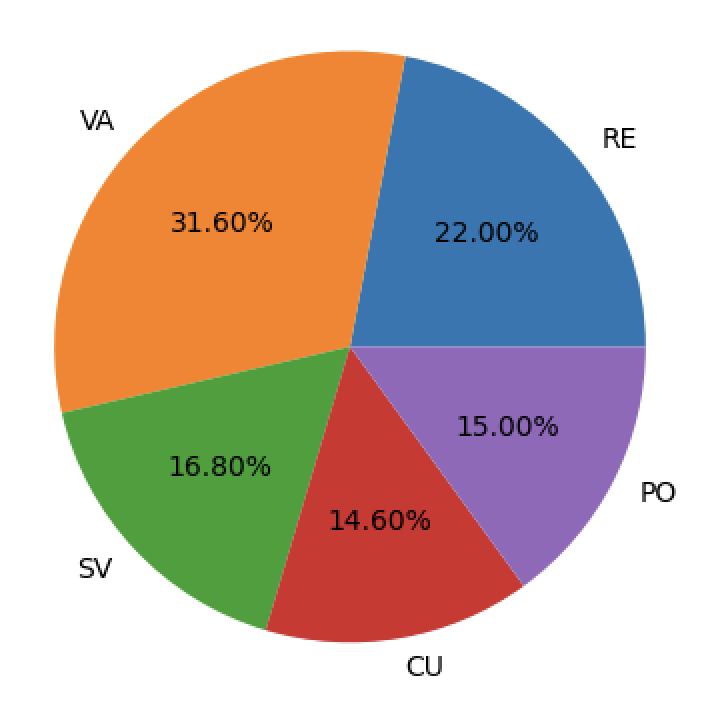
\includegraphics[scale=0.4]{top_dist.png}
    \caption{Topic distribution of all tweets}
    \label{fig:top-dist}
\end{figure}
\begin{figure}[H]
    \centering
    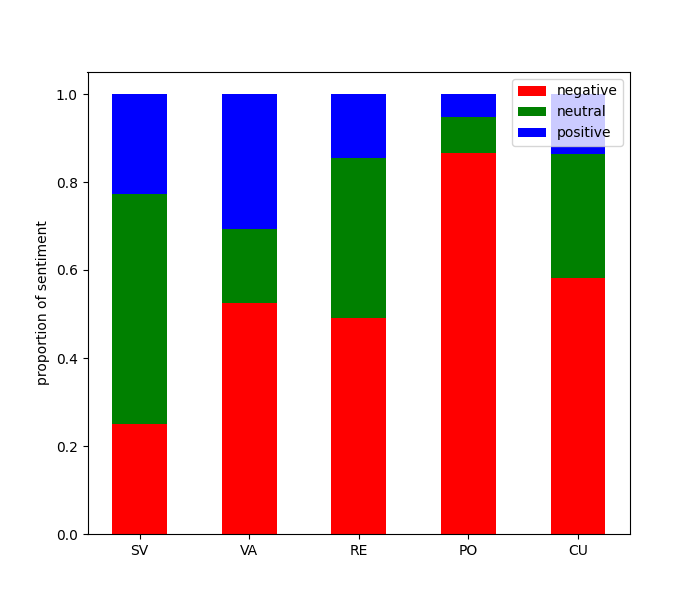
\includegraphics[scale=0.5]{topic_sentiment.png}
    \caption{Sentiment distribution for each topic}
    \label{fig:sent-top-dist}
\end{figure}
The 10 most relevant words to each topic is the 10 words with the highest tf-idf score for that topic. The 10 most relevant words to each topic are represented in Table \ref{table1}. \par
\begin{table*}[t]\centering
\begin{tabular}{cccccc}
\hline
\# & SV              & VA              & RE           & PO              & CU              \\ \hline
1  & ``omicron"    & ``booster"         & ``mask"   & ``trump"       & ``market"        \\ \hline
2  & ``variant"        & ``omicron"      & ``health"      & ``biden"       & ``health"        \\ \hline
3  & ``coronavirus" & ``virus"         & ``omicron"  & ``government" & ``impact"        \\ \hline
4  & ``symptoms"         & ``shot"       & ``virus" & ``vax"    & ``pandemic"       \\ \hline
5  & ``africa"         & ``mrna"       & ``mandatory"    & ``anti"       & ``life"         \\ \hline
6  & ``virus"     & ``die"    & ``mandate" & ``fauci"        & ``omicron" \\ \hline
7  & ``health"          & ``unvaccinated"          & ``test"  & ``unvaccinated"    & ``help"     \\ \hline
8  & ``mild"      & ``deaths"      & ``spread"    & ``virus"      & ``variant"       \\ \hline
9  & ``infected"       & ``health" & ``workers"   & ``world"         & ``christmas"         \\ \hline
10 & ``infection"      & ``effects"       & ``variant"      & ``family"         & ``media"         \\ \hline
\end{tabular}
\caption{Words with top 10 highest tf-idf scores for each topic.}
\label{table1}
\end{table*}
In order to inform our analysis of the top 10 most relevant words for each topic, we want to study the sentiment of the tweets where the top 10 most relevant words are mentioned. This allows us to determine whether these words are said in a positive light or a negative light, and allow us narrow down on which subtopics within each topic are the most contentious. The sentiment distribution of the top 10 most relevant words in COVID Severity (SV), COVID Vaccination (VA), COVID Response (RE), COVID Politics and Discourse (PO) and COVID Culture (CU) is in Figures \ref{fig:sv-dist}, \ref{fig:va-dist}, \ref{fig:re-dist}, \ref{fig:po-dist}, \ref{fig:cu-dist} respectively. \par
\begin{figure}[H]
    \centering
    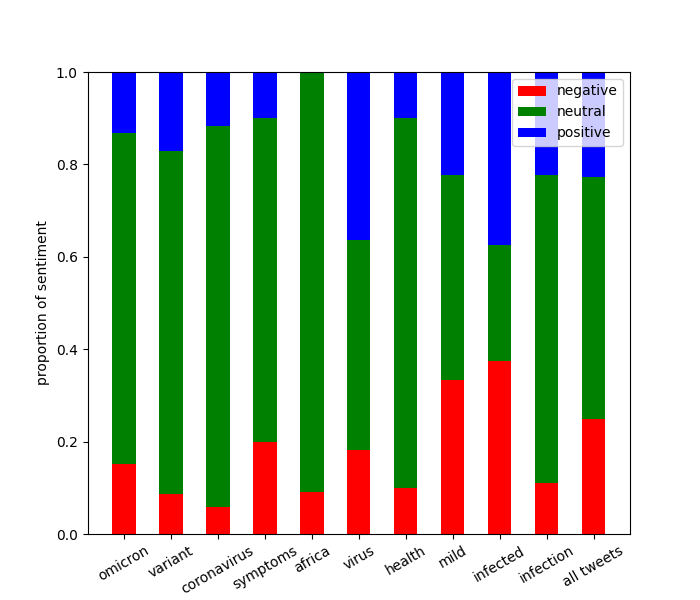
\includegraphics[scale=0.45]{SV_word_sentiment.png}
    \caption{Sentiment distribution of most relevant words in COVID Severity (SV)}
    \label{fig:sv-dist}
\end{figure}
\begin{figure}[H]
    \centering
    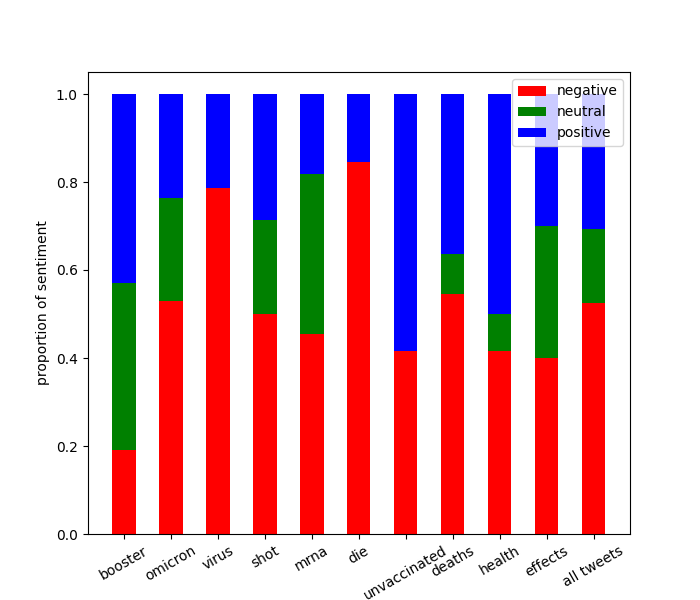
\includegraphics[scale=0.45]{VA_word_sentiment.png}
    \caption{Sentiment distribution of most relevant words in COVID Vaccination (VA)}
    \label{fig:va-dist}
\end{figure}
\begin{figure}[H]
    \centering
    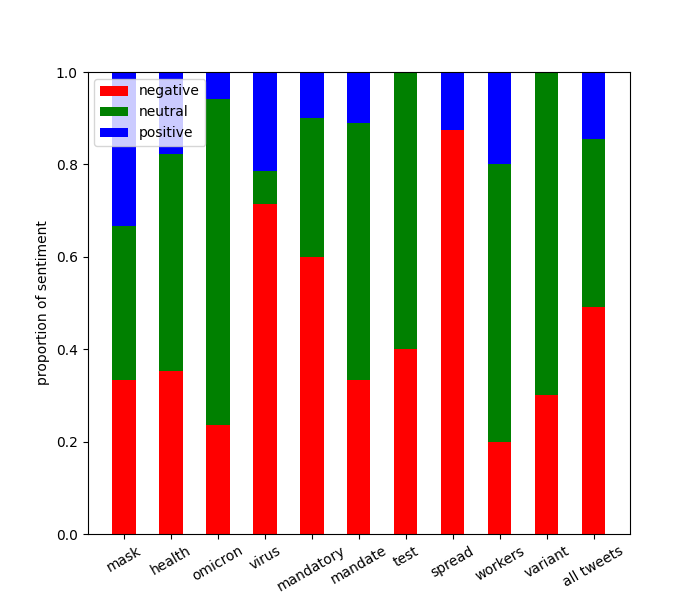
\includegraphics[scale=0.45]{RE_word_sentiment.png}
    \caption{Sentiment distribution of most relevant words in COVID Response (RE)}
    \label{fig:re-dist}
\end{figure}
\begin{figure}[H]
    \centering
    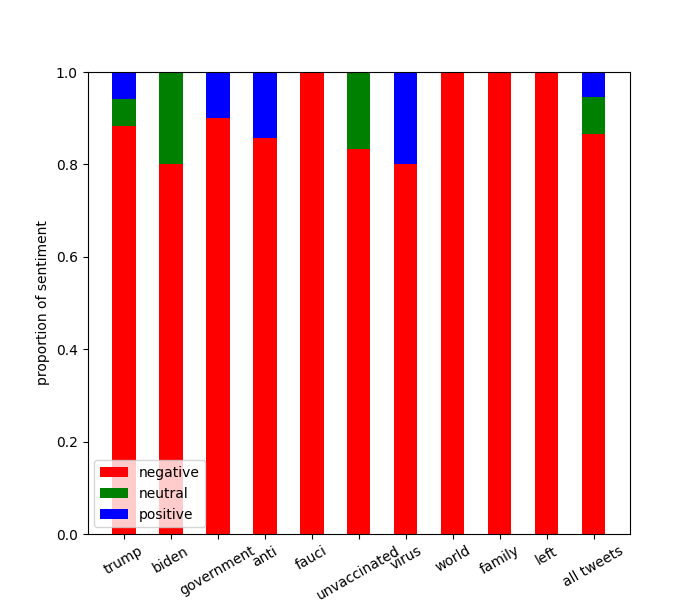
\includegraphics[scale=0.45]{PO_word_sentiment.png}
    \caption{Sentiment distribution of most relevant words in COVID Politics and Discourse (PO)}
    \label{fig:po-dist}
\end{figure}
\begin{figure}[H]
    \centering
    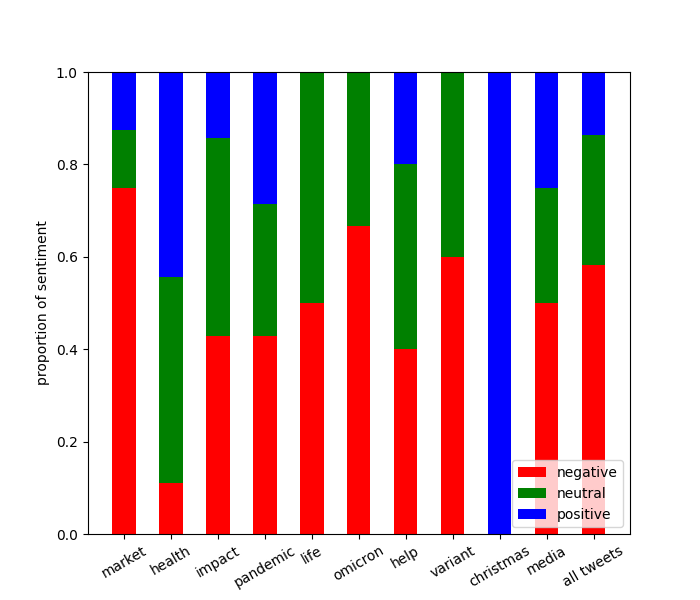
\includegraphics[scale=0.45]{CU_word_sentiment.png}
    \caption{Sentiment distribution of most relevant words in COVID Culture (CU)}
    \label{fig:cu-dist}
\end{figure}
From Table \ref{table2}, we have the list of top 10 most relevant words for each topic that are coded more positively or negatively than the average sentiment for that topic. This informs our inference on the content of negative and positive tweets.
\begin{table*}[t]
\centering
\begin{tabular}{ccc}
\hline
Topic & More negative than average                                                                                   & More positive than average                                                                                            \\ \hline
SV    & ``omicron", ``symptoms", ``africa", ``mild"                                                                  & \begin{tabular}[c]{@{}c@{}}``variant", ``coronavirus", ``virus", ``health", \\ ``infected", ``infection"\end{tabular} \\ \hline
VA    & ``omicron", ``virus", ``shot", ``mrna", ``die"                                                               & \begin{tabular}[c]{@{}c@{}}``booster", ``unvaccinated", ``deaths",\\  ``health", ``effects"\end{tabular}              \\ \hline
RE    & \begin{tabular}[c]{@{}c@{}}``omicron", ``mandatory", ``test", \\ ``spread", ``variant"\end{tabular}          & \begin{tabular}[c]{@{}c@{}}``mask", ``health", ``virus", \\ ``mandate", ``workers"\end{tabular}                       \\ \hline
PO    & \begin{tabular}[c]{@{}c@{}}``biden", ``fauci", ``unvaccinated", ``world", \\ ``family", ``left"\end{tabular} & ``trump", ``government", ``anti", ``virus"                                                                            \\ \hline
CU    & ``market", ``life", ``omicron", ``variant"                                                                   & \begin{tabular}[c]{@{}c@{}}``health", ``impact", ``pandemic", \\ ``help", ``christmas", ``media"\end{tabular}         \\ \hline
\end{tabular}
\caption{Top 10 words said more positively or negatively than average}
\label{table2}
\end{table*}
\section{Discussion}
% \textit{1 page. interpret your results in terms of what they reveal about the way each candidate was being discussed and perceived. Make extensive use of your results to justify your interpretations.}
Figure \ref{fig:top-dist} above implies that the most popular topic from our Twitter data with our given query was VA. This makes sense given our query terms are all related to vaccination. The second most popular topic was RE, which also makes sense given our query terms, since vaccine mandates were categorised under RE. Other than that, relative engagement in each topic is roughly the same. People seem equally engaged in discussing all facets of COVID affecting their lives, from infection severity to the government's response to political discussion. \par
Figure \ref{fig:sent-top-dist} above implies the following, on average. People are split on whether or not COVID is severe. People have a negative response towards vaccination and the COVID vaccine. People do not approve of the COVID response from governments. People have a lot of negative sentiment when expressing political views, indicating a high degree of polarisation and that COVID is a partisan issue. Finally, people have a lot of negative sentiment when discussing culture surrounding COVID, implying that COVID has a strongly negative impact on their daily life. \par
From Table \ref{table1}, we have the top 10 most relevant words characterising discussion within each topic. However, people can use the same words to argue for and against the topics. For example, ``symptoms" under SV can be used to argue that symptoms of COVID are mild, and thus COVID is not severe. At the same time, ``symptoms" can also be used to argue that symptoms of COVID are very serious, and thus COVID is severe. In order to differentiate between these two connotations of the usage of words, we computed the positive/neutral/negative sentiment for all of the top 10 most relevant words for each topic, as shown in Figures \ref{fig:sv-dist}, \ref{fig:va-dist}, \ref{fig:re-dist}, \ref{fig:po-dist}, \ref{fig:cu-dist}. From there, for each word, we compare the ratio of negative sentiment to positive sentiment of that word under that given topic to the ratio of negative sentiment to positive sentiment for all tweets under that topic. We then categorise the top 10 most relevant words for each topic into ``more negative than average" and ``more positive than average", as shown in Table \ref{table2}. This allows us to narrow down our analysis to the exact arguments that people with negative and positive sentiment make respectively. \par
Under the topic SV, we can see that those who do not believe that COVID is severe use the words ``omicron", ``symptoms", ``africa" and ``mild". We can infer that they believe that getting COVID only results in mild symptoms, and are citing the recent Omicron variant from South Africa to back up their claims. We can see that those who believe that COVID is severe use the words ``variant", ``coronavirus", ``virus", ``health", ``infected" and ``infection". We can infer that they are afraid of getting infected by COVID variants which would impair their health. \par
Under the topic VA, those who do not approve of the COVID vaccine use the words ``omicron", ``shot", ``mrna" and ``die". We can infer that they are afraid of dying from the COVID vaccine, they are concerned about the fact that the COVID vaccine is an mRNA vaccine, and they are citing the Omicron variant, which recent research has shown might not be as effective against the COVID vaccine, as evidence. Those who approve of the COVID vaccine use the words ``booster", ``unvaccinated", ``deaths", ``health", and ``effects". We can infer that those who approve of the vaccines cite deaths and health effects, they are in favour of booster shots, and are concerned about the unvaccinated population. \par
Under the topic RE, those who do not approve of the COVID response use the words ``omicron", ``mandatory", ``test", ``spread", and ``variant". Lack of approval of the COVID response comes in two types: those who believe that the restrictions are too tight, and those who believe that the restrictions are too lax. We thus know that the contentious topics are the spread of the newly discovered Omicron variant, COVID testing and mandatory restrictions like mandatory vaccinations. However, we cannot infer anything further about whether they are for or against restrictions, just that they are dissatisfied by the current state of affairs. Those who approve of the COVID response use the words ``mask", ``health", ``virus", ``mandate" and ``workers". We can infer that they approve of mask mandates and COVID response for workers, and are concerned about their health and the virus.\par
Under the topic PO, those express political views with negative language use the words ``biden", ``fauci", ``unvaccinated", ``world", ``family" and ``left". We can infer that the negative political sentiment is concentrated on political figures Democrat US President Joe Biden, US Chief Medical Advisor to the President Anthony Fauci. Other negative political sentiment is directed towards the ``left", which is a term for the liberal party in the US, as well as the unvaccinated. Negative political sentiment towards the world in general can be interpreted as inter-country tensions. Those who express political views with positive language use the words ``trump", ``government", ``anti", and ``virus". This implies that there is positive political sentiment being expressed on Republican Former US President Donald Trump, as well as the government. This positive political sentiment is driven in some way by the virus. \par
Under the topic CU, those that express cultural views surrounding COVID with negative language use the words ``market", ``life", ``omicron" and ``variant". We can infer that the negative cultural impact due to COVID are concentrated around the economy and markets, as well as people's daily lives, and that the Omicron variant is in part responsible for this. Those that express cultural views surrounding COVID with positive language use the words ``health", ``impact", ``pandemic", ``health", ``christmas", and ``media". We can infer that the positive cultural impacts of COVID is related to Christmas, which has not been stalled due to the pandemic, as well as the media, and people helping one another. \par
From all of the inference we have made above, we can see that people have a general negative response to the pandemic and vaccination. If one does not believe in the severity of COVID, the government response can seem extremely overblown. If one really believes in the severity of COVID, the government response can seem insufficient. Either way, lockdowns, market instability, inflation and COVID infection is affecting everyone's daily lives. Beyond that, since COVID has become a partisan topic, political discussions about COVID are overwhelmingly negative and hostile. \par
The negative response to vaccination comes from the fear of dying from the vaccine, the new technology of the mRNA vaccine, and how the vaccine is less effective on the Omicron variant. Furthermore, those who believe that COVID is not severe do not see the need of vaccinations when they believe that COVID symptoms are mild. Vaccine status has also clearly become a partisan topic, as it is amongst the top 10 most relevant words in political discussion. This means that there can be further negative response to the vaccine due to political beliefs. 
\section{Group Member contributions}
% \textit{0.25 page.  a description of the contributions each group member made to this project.}
\begin{itemize}
  \item Tiffany Yong
    % \subsection{Tiffany Yong}
    \begin{itemize}
        \item Planning of the project, distribution of tasks. 
        \item Data annotation: Performed open coding; chose, modified, and finalized topics; proceeded to complete manual data annotation.
        \item Report writing: Wrote introduction, results and discussion
    \end{itemize}
  \item Youyuan Zhang
    \begin{itemize}
        \item Data collection: Collected raw data from Twitter, proceeded to filter non-trivial entries of data for annotation, created data set of randomly selected entries for open coding.
        \item Data analysis: Computed 10 words in each category with highest TF-IDF score.
        \item Report writing: Wrote data
    \end{itemize}
  \item Yufeng Peng
    \begin{itemize}
        \item Data annotation: Assisted in modifying and finalizing the topics in the stage of open coding.
        \item Report writing: Set up the AAAI format of the project report and wrote methods
    \end{itemize}
\end{itemize}
\bibliography{main.bib}
\end{document}
